\documentclass{standalone}
\usepackage{tikz}
\usepackage{verbatim}
\usepackage{skull}
\usepackage{tikzsymbols}
\begin{document}
\pagestyle{empty}
  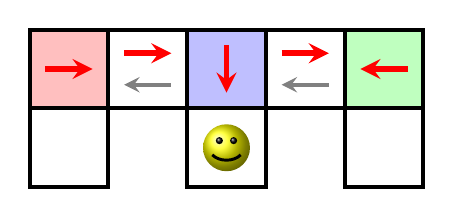
\begin{tikzpicture}
  \node[draw,rectangle, fill=red!25, line width=0.5mm, minimum width = 1cm, minimum height = 1cm] at (0,0) {};
  \node[draw,rectangle, fill=none, line width=0.5mm, minimum width = 1cm, minimum height = 1cm] at (1,0) {};
  \node[draw,rectangle, fill=blue!25, line width=0.5mm, minimum width = 1cm, minimum height = 1cm] at (2,0) {};
  \node[draw,rectangle, fill=none, line width=0.5mm, minimum width = 1cm, minimum height = 1cm] at (3,0) {};
  \node[draw,rectangle, fill=green!25, line width=0.5mm, minimum width = 1cm, minimum height = 1cm] at (4,0) { };
  
  \node[draw,rectangle, fill=none, line width=0.5mm, minimum width = 1cm, minimum height = 1cm] at (0,-1) {\large $\skull$};
  \node[draw,rectangle, fill=none, line width=0.5mm, minimum width = 1cm, minimum height = 1cm] at (2,-1) {\Huge $\dSmiley$};
  \node[draw,rectangle, fill=none, line width=0.5mm, minimum width = 1cm, minimum height = 1cm] at (4,-1) {\large $\skull$};
  
  \draw[-stealth, line width=.75mm, color=red] (-0.3,0) -- (0.3,0);
\draw[-stealth, line width=.75mm, color=red] (2.,0.3) -- (2.,-0.3);
\draw[stealth-, line width=.75mm, color=red] (3.7,0) -- (4.3,0);

\draw[-stealth, line width=.75mm, color=red] (0.7,0.2) -- (1.3,0.2);
\draw[stealth-, line width=.5mm, color=gray] (0.7,-0.2) -- (1.3,-0.2);

\draw[-stealth, line width=.75mm, color=red] (2.7,0.2) -- (3.3,0.2);
\draw[stealth-, line width=.5mm, color=gray] (2.7,-0.2) -- (3.3,-0.2);

  \end{tikzpicture}
\end{document}